%!TEX root = predictability.tex

\section{Identifying the Main Sources\\ of Variance}
Database Management Systems are very complex systems, and there are many
possible sources of variance, such as I/O operations, locking, thread
scheduling, etc. There are tools to gather information about these events.
For example, using strace, you can collect data about every I/O operation
including size of data read or written, time of each I/O operation, etc.
However, such kind of information is not intuitive enough for explaining
the variance of latency even for the most skilled database administrators.
Moreover, these tools are usually related to the kernel, thus introducing
overhead such as context switching for each system call. This could be quite 
expensive and would also introduce noise into the latency data. These tools,
therefore, are not suitable for analyzing the source of variance. We tackle
this problem using a different approach.

\subsection{Variance Break Down}
The latency of a transaction is the time it takes to process a transaction, and
the processing of a transaction can be traced down to some high level function 
in the system's source code that is responsible for executing the queries. In
MySQL, this high level function is called \texttt{dispatch\_command}.
Therefore, the latency of a transaction is basically the execution time of this 
high level function during a transaction, and the variance of latency is the
variance of the execution time of this function in different transactions.

\begin{figure*}
\centering
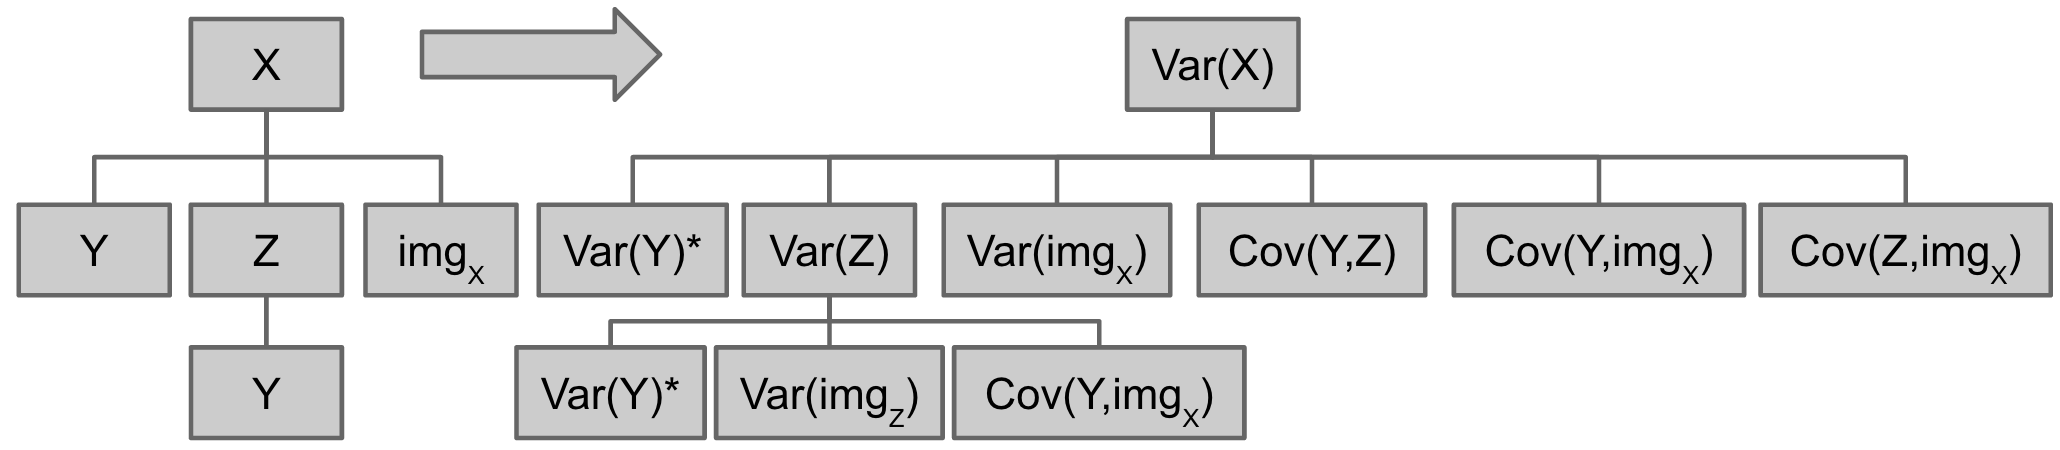
\includegraphics[scale=0.5]{plots/var_break_down}
\caption{A static call graph and its corresponding \textit{variance tree}}
\label{fig:var_break_down}
\end{figure*}

Most of the time, a function has to call other functions to accomplish its
job. A function's execution time is roughly the total execution time of all
the functions it calls. In this paper, we refer to the function that calls
other functions as the \textit{parent function}, and those being called as the
\textit{child functions} of it. For example, if function X calls function Y and
Z, then X would be the \textit{parent function} of Y and Z and they would
be the \textit{child functions} of X. Let $E(f)$ denote the execution time of
function f, we have
\begin{displaymath}
E(X) = E(Y) + E(Z)
\end{displaymath}

However, strictly speaking, this is incorrect because besides calling function
Y and Z, function X also has to execute some other basic statements, like
variable assignments, if statements, etc. The time spent on them, although
might be way smaller than the time spent on function Y and Z, must also be
considered. To model this, we can add an \textit{imaginary function} $img_X$
to the list of children of X. In this way, we can now say that function X does
nothing other than calling function Y, Z and $img_X$, and so
\begin{displaymath}
E(X) = E(Y) + E(Z)+ E(img_X)
\end{displaymath}

Let's say $E(X)$ has a large variance and we would like to know why. Since the
only thing X does is invoking function Y, Z and $img_X$, we know that one or
more of these functions are to blame for the variance. To find out the 
functions that cause $E(X)$ to have a large variance, we need to quantify
the contribution of each and every \textit{child function} of X.

Variance can be calculated in many ways, the following one being one of them:
\begin{equation}
Var(\sum_{i=1}^{n}X_i) = \sum_{i=1}^{n}Var(X_i) + 2\sum_{1\leq i}\sum_{\leq j \leq n}Cov(X_i, X_j)
\label{eq:var-break-down}
\end{equation}
Using this formula, we can easily break down the variance of $E(X)$ into the
variances and covariances of the execution time of function Y, Z and $img_X$,
in which the variances can be further broken down by applying the same formula.
For the rest of this paper, we use the term ``variance of a function'' as an
abbreviation for the variance of the execution time of a function, and the term
``covariance of two functions'' as the abbreviation for the covariance of two
functions' execution time for simplicity. Figure \ref{fig:var_break_down} shows
the result of breaking down the variance of X. The graph on the left is the
static call graph, which shows that function X calls functions Y, Z, and $img_X$.
The graph on the right shows that the variance of X can be broken down into
the variances of Y, Z, $img_X$, and the covariances of every two of them. It
also shows how the variance of Z can be further broken down. We call this graph
a \textit{variance tree}.

Variance break down is fairly easy to do with the source code. Given a 
function, we can inserted a small piece of code into the source code of this
function to retrieve the timestamp at the beginning and end of this function,
and then calculate its execution time using these two timestamps easily. 
Similarly, for each function call in this function, we retrieve the timestamp
before and after the function call and calculate the execution time 
accordingly.

Applying this technique on the functions in MySQL responsible for query
processing allows us to see each function's contribution to the overall
variance and locate those with significant contributions. Looking only at the
value of variance or covariance is not enough, though. An obvious example is
that function \texttt{dispatch\_command} contributes to 100\% of the variance
of latency, but it barely gives us any useful information about the cause of
the variance. This means that we also need to consider how useful a function is
in helping us find out the actual cause behind the high variance.

Another thing to notice is that, a function can be called in different places
in the source code, so there can be multiple nodes in the \textit{variance
tree} that represent the variance of the same function or the covariance of the
same functions, each with a possibly different value. For example, in figure
\ref{fig:var_break_down}, both function X and Z calls function Y, and so in the
\textit{variance tree}, there are two nodes that both represent the variance of
function Y(marked with asterisk). It is possible that to reduce the variance X,
we need to change the implementation of Y, which would affect the values of
both nodes. Therefore, we must consider them all together. We use the term
\textit{factor} to represent the variance of a function or the covariance of
two functions during the execution of a transaction. On the other hand, the
nodes in the \textit{variance tree} represents the variance of a function or
the covariance of two functions only during the execution of some particular
function. We call them the \textit{instances} of the \textit{factor}. Each
node in the \textit{variance} corresponds to an \textit{instance}. In figure
\ref{fig:var_break_down}, Var(Y) is a \textit{factor}, and the two nodes marked 
with asterisks in the \textit{variance tree} are \textit{instances} of
\textit{factor} Var(Y).

The goal of finding the main sources of variance in transaction latency
now turns into finding the \textit{factors} such that:

\begin{itemize}
    \item make significant contributions to the variance of transaction latency
    \item give us enough information about the cause of variance
\end{itemize}

\subsection{Factor Selection}
To select \textit{factors} that satisfy the two criteria mentioned above, we 
need to quantify them. The first one can be quantified by the value of variance 
or covariance. For the rest of this paper, we use the term 
\textit{contribution} to represent the value of variance of covariance. An
intuition to quantify the second criterion is that, the more specific a
function is about what it does, the more information it can
give us about the cause of its variance. Moreover, a \textit{child function} is
usually more specific about its job than its \textit{parent function}.

For example, a function A that writes several log records to the global log
buffer must first acquire the lock on the log buffer(function B), copy the
log data to the log buffer(function C), and finally release the
lock(function D). Let us say function A's variance is 30\% of the
variance of latency and function C's variance is 28\% of the variance
of latency. We would find function C more interesting than function A
because even though its variance is smaller than that of function A, it
has narrower functionality and is more specific. It's possible that a closer
look at this function can tell us that its variance is caused by the size of
log data being copied to the log buffer each time, and so a solution that
reduces log size variance could effectively reduce the overall variance.

Therefore, the ``specificness'' of a \textit{factor} is related to the
heights of the functions involved. Also, given a call graph, no matter how 
many different places a function occurs, all these nodes have the same 
height. We can use existing call graph generation tools likes CodeViz
\footnote{http://www.csn.ul.ie/\textasciitilde{}mel/projects/codeviz/} to
generate the call graph and pre-compute the height of any given function. Most
of the time, the smaller the height is, the more specific the function is about
what it does. With this intuition, we can define the ``specificness'' of a
\textit{factor} as a decreasing function of the heights of the functions
involved. In our experiments, we use the following function:
\begin{equation}
speci(N) = (height(call\_graph) - height(N))^3
\label{eq:speci}
\end{equation}
In this function, $height(call\_graph)$ is the height of the sub call graph
whose root is function \texttt{dispatch\_command}. $height(N)$ is the height of 
the function if $N$ represents the variance of function, and the larger height
if $N$ represents the covariance of two functions.

Now we can define the responsibility of a \textit{factor} to the overall
transaction latency as
\begin{equation}
resp(N) =  speci(N)\sum_{i}contri(N_i)
\label{eq:resp}
\end{equation}
where N is a \textit{factor} and $N_i$ are \textit{instances} of this
\textit{factor} in the \textit{variance tree}.

\begin{algorithm}[t]
    \SetAlgoLined
    \SetKwInOut{Input}{Inputs}
    \SetKwInOut{Output}{Output}
    \SetKwFunction{FactorOf}{factor\_of}
    \SetKwFunction{NewFactor}{new\_factor}
    \SetKwFunction{Speci}{speci}
    
    \Input{
        $t$, variance break-down tree,\\
        $k$: maximum number of functions to select,\\
        $d$: threshold for minimum contribution}
        
    \Output{
        $s^*$: top $k$ most responsible factors}
    \BlankLine
        
    $h \gets $ empty list\;
    \BlankLine    
    
    \ForEach{$ node~ N \in t$} {
        $N^* \gets \FactorOf{h, N}$\;
        \uIf{$N^* = NULL$} {
            $N^* \gets \NewFactor{}$\;
            $N^*.contri \gets 0$\;
            $h \gets h \cup N^*$\;
        }
        \uElse{
            $N^*.contri \gets N^*.contri + N.contri$\;
        }
    }
    \BlankLine    
    
    \ForEach{$N^* \in h$} {
        $N^*.resp = \texttt{speci}(N^*) \cdot N^*.contri$\;
    }
    \BlankLine
    
    Sort $h$ in descending order of $N^*.resp$\;
    \BlankLine
    
    $s^* \gets$ empty list\;
    \For{$ i \gets 1$ \KwTo $k$} {
        $N^* \gets h[i]$\;
        \uIf{$N^*.contri \geq d$} {
            $s^* \gets s^* \cup N^*$\;
        }
        \uElse{
            break\;
        }
    }
    
    \KwRet{$s^*$}\;
    
\caption{Factor Selection}
\label{alg:factor-selection}
\end{algorithm}

Given the \textit{variance tree}, we now propose an algorithm to select the top
k most responsible \textit{factors} from this tree for the variance of latency.
The pseudocode is shown in algorithm \ref{alg:factor-selection}. The basic
idea of this algorithm is very simple. We iterate over the \textit{variance 
tree}, and for each node, and check if the \textit{factor} of this node is 
already in list $h$. If not, we add the \textit{factor} to $h$. If the
\textit{factor} is already in $h$, we need to add the contribution of this
node(the value of variance of covaraince) to the contribution \textit{factor}
(line 1 to line 10). After we find all \textit{factors}, we calculate their
\textit{resp} values using equation \ref{eq:resp} (line 11 to 13). After that,
we sort the \textit{factors} in descending order of their \textit{resp} values,
and select the ones with a total contribution value greater than or equal to
threshold $d$ from the first $k$ elements of list $h$(line 14 to 23).

\subsection{VProfiler: A Variance Source Discovery Framework}

\begin{algorithm}[t]
    \SetAlgoLined
    \SetKwInOut{Input}{Inputs}
    \SetKwInOut{Output}{Output}
    \SetKwFunction{VarBreakDown}{var\_break\_down}
    \SetKwFunction{SetRoot}{set\_root}
    \SetKwFunction{AddChildren}{add\_children}
    \SetKwFunction{SelectFactors}{select\_factors}
    \SetKwFunction{NeedsBreakDown}{needs\_break\_down}
    \SetKwFunction{GetInstanceOf}{get\_instance\_of}
    \SetKwFunction{IsVariance}{is\_variance}
    \SetKwFunction{Clear}{clear}
    
    
    \Input{
        $v$: variance of function $dispatch\_command$,\\ 
        $k$: maximum number of functions to select,\\
        $d$: threshold for minimum contribution,\\
        $m$: threshold for minimum relatively contribution of children}
        
    \Output{
        $s^*$: top $k$ most responsible factors}
    \BlankLine
        
    $t \gets$ empty tree\;
    $t.\SetRoot{v}$\;
    $l \gets$ empty list\;
    $l \gets l \cup v$\;
    $e \gets true$\;
    \BlankLine
    
    \While{$e$} {
        \BlankLine
        
        \ForEach{$factor~ f \in l$} {
            \If{$\IsVariance{f}$} {
                \ForEach{$instance~ i \in f$} {
                    $c \gets \VarBreakDown{i}$\;
                    $t.\AddChildren{i, c}$\;
                    \ForEach{$child~ n \in c$} {
                        \If{$n.contri / i.contri \geq m$} {
                            $i.contri = 0$\;
                            break\;
                        }
                    }
                }
            }
        }
        \BlankLine
        
        $s^* \gets \SelectFactors{t, k, d}$\;
        \BlankLine
        
        $l.\Clear{}$\;
        $e \gets false$\;
        \ForEach{$factor~ f \in s^*$} {
            \uIf{$\NeedsBreakDown{f}$} {
                $l \gets l \cup f$\;
                $e \gets true$\;
            }
            \uElseIf{$\IsVariance{f}$} {
                $h \gets \GetInstanceOf{t, f}$\;
                $h.contri \gets \infty$\;
            }
        }
        \BlankLine
    }
    
    \KwRet{$s^*$}\;
    
\caption{Work-flow of VProfiler}
\label{alg:iterative-selection}
\end{algorithm}

The \textit{factor\ selection} algorithm introduced above describes how to
select the top k most responsible \textit{factors} from a given
\textit{varaince tree}. Now we introduce a framework to identify the main
sources of variance in MySQL(or other applications). We call it VProfiler,
which works as follows:\\\\
\textbf{Initialization(Algorithm \ref{alg:iterative-selection}, line 1 to 5)}

VProfiler starts with an empty \textit{variance tree}, and then it uses the
variance of the top level function \texttt{dispatch\_command} as the root.
VProfiler also maintains a list of \textit{factors} that need to be further
broken down(list $l$ in the algorithm). This list contains only the
\textit{factor} Var(\texttt{dispatch\_command}) at the beginning.\\\\
\textbf{Variance Break Down(Algorithm \ref{alg:iterative-selection}, line 7 to
12)}

For each factor that needs to be broken down, VProfiler finds out all its
\textit{instances} in the \textit{variance tree}, and break each one down by
modifying the source code and calculating the execution time of the functions
using timestams. It then adds these nodes to the \textit{variance\ tree} as the
children of the corresponding node. In this way, the \textit{variance tree}
is gradually expanded.

There's one more situation we need to take care of. Using the previous example
of function X, Y and Z, if the variance of X is 300 and the variance of Y is
285, then obviously we need to only focus on Y, and function X can be safely
ignored. VProfiler does the similar thing. After it breaks down some
\textit{instance} of a \textit{factor}, it first checks if any of the variance
or covariance of its \textit{child functions} takes a significant portion of
the \textit{instance}'s variance value using $m$ as the threshold. If so, it
sets the \textit{contri} value of this \textit{instance} to 0 because it
becomes unimportant.\\\\
\textbf{Factor Selection(Algorithm \ref{alg:iterative-selection}, line 13 to
23)}

After the \textit{variance tree} is expanded, VProfiler does a \textit{factor
selection} to choose the top k most responsible \textit{factors} for the
overall variance. Then, it provides the selected \textit{factors} to the
users, who needs to look at each selected \textit{factor}. If it is the
variance of a function, the users needs to look at the implementation of the 
function and see if it tells them enough information about the cause of the 
variance. If not, then they need to ask VProfiler to further break down its
variance. VProfiler then add it to the list $l$. If this function reveals the
cause of its variance, the users notify VProfiler that it's selected
(Now that the users already understand the cause of its variance, this
function definitely gives them ``enough'' information). VProfiler picks one of
its \textit{instances} in the \textit{variance tree} and set its contribution
to infinity to make sure that it will finally be selected. If there is any
function that needs to be further investigated, VProfiler will continue
this select-investigate loop until it finally finds out k(or less)
factors that could explain the variance of latency.

Note that the factors finally returned by VProfiler are only meant to point out
some functions that are highly related to the variance of latency. Close
analysis is still needed to finally locate the actual problem. For example,
although a factor takes into consideration the sum of all its 
\textit{instances}, it could also be the case that only one or two
\textit{instances} matter while the contributions of the rest are negligible.
The actual cause of variance, therefore, might be related to these important
\textit{instances} instead of the implementation of the function.

\subsection{DTrace v.s. VProfiler}
DTrace, which stands for \textit{Dynamic Tracing}, is a very powerful tracing
framework which can be used for performance analysis and troubleshooting on all
softwares, including user-level applications like database and also kernel-
level programs like operating system kernels and device drivers. DTrace is used 
in an event-listener manner --- users specifies the event they want to listen
to, along with a piece of code which will be executed when the specified event
occurs. Multiple events can be specified at the same time, each called a
\textit{probe} in DTrace. Different types of probes are provided by different
\textit{providers}. For example, the \textit{syscall} provider provides probes
related to system calls, like the start and exit of the \texttt{open} system
call.

The \textit{pid} provider of DTrace allows users to dynamically patch running
processes with instrumentation code without touching the static files on the 
disk or restarting the programs. The following is an example of a probe of the
\textit{pid} provider:

$pid:module:function\_name:\{entry, return\}$

This probe contains 4 fields, all of which can be omitted except the first one.
The first field specifies the ID of the target process. The second field is
the name of the module the target function is in, such as $mysqld$ or $libc$.
The third field is the name of the target function, which can be either the
exact name or can contain wildcard characters like ``*'' and ``?''. The fourth
field should be one of entry and return, which denote the start event and
exit event of the target function, respectively. When any filed is omitted, it
means ``match anything possible''. Particularly, when the last filed is
omitted, it matches both the entry probe and the return probe as well as
instruction probes, which are fired for each CPU instruction executed.

Using the probes provided by the \textit{pid} provider, we can also use DTrace
to measure the execution time of a \textit{parent function} and its
\textit{child functions}, therefore breaking down the variance of the
\textit{parent function} using formula \ref{eq:var-break-down}.

Despite its great power in tracing both user-space and kernel-space programs
and its convenience in patching running processes, there are several reasons
why VProfiler is better than DTrace.

First of all, DTrace was originally developed for Solaris, and gained support
by other Unix-like systems, including FreeBSD, Mac OS X, Open Solaris.
Unfortunately, it's one of the tools that are not shared between Linux and Unix
systems. The only Linux system that offers official DTrace support is Oracle
Linux. However, neither Oracle Linux nor Unix is among the popular operating
system people would choose for their servers. Popular cloud virtual machine
platforms like Amazon EC2 and Microsoft Azure no longer support Unix systems.
Moreover, even through DTrace is supported by Oracle Linux, a subscription
account is needed to use it, which is not free. There is an unofficial port of
DTrace for Linux \footnote{https:// github.com/dtrace4linux/linux}. However,
up until now \footnote{Feb. 2, 2015} its \textit{pid} provider is pretty much
broken, and DTrace crashes when it tries to execute any DTrace script or
command containing \textit{pid} probes.

Second, the script language DTrace uses has very limited language feature. It's
dynamically typed, and does not support user-defined data type or function.
What's worse, although this language supports attaching predicates to probes to
decide whether or not the probes will be executed, it does not have any flow
control statement like if statement or loop statement, making complex code
impossible. DTrace matches functions by name. Therefore, when one function is
called at multiple places of another function, it's very difficult to
distinguish them in DTrace unless instruction probes are used, which would be
very expensive. Moreover, when tracing the execution time of functions, we
need to record the execution time of each \textit{child function} in each
transaction. To store all these data, we have to use the built-in 
\textit{associative array} data type, whose performance depends on the
implementation of DTrace. Even if its overhead is too huge, there is nothing
the users can do to improve its performance. On the contrary, in VProfiler, we
can always try to find more efficient data types or use faster algorithms to
make the overhead of tracing as small as possible. Experiment results that
compares the overhead of VProfiler and DTrace are shown in section 6.6.1. 

Third, even if one buys a high end server to run Solaris on it, and writes the
most efficient DTrace script for tracing functions, it is still possible that
DTrace will disappoint the user. In our experiments with DTrace, we found that
some of the return probes are lost. It turns out to be a known issue of 
DTrace \cite{brendan:dtrace}. This can happen when the target function is very
complex and the compiler optimizes it using jump table, which makes it
difficult for DTrace to dissemble the instructions and correctly locate the
return points.



